\documentclass{beamer}

\usepackage{tikzducks}
\usepackage{tikzlings}

\setbeamertemplate{navigation symbols}{}
\setbeamertemplate{background canvas}{
\includegraphics[height=\paperheight]{Background}}

\usepackage{xfp}
\ExplSyntaxOn
\let\intmodnn\int_mod:nn
\ExplSyntaxOff

\newcommand{\tourist}{%
\ifnum \intmodnn{\thepage}{10} > 5
	\marmot[
		rightstep,
		scale=1.6, 
		xshift=3cm, 
		yshift=-3.4cm,
		book={\tiny Guide},
		bookcolour=violet!50!red,		
	]
\else
	\marmot[
		leftstep,
		scale=1.6, 
		xshift=3cm, 
		yshift=-3.4cm,
		book={\tiny Guide},
		bookcolour=violet!50!red,		
	]
\fi
	\thing[
		scale=1.5, 
		xshift=3.7cm, 
		yshift=-3.45cm,
		strawhat=red!50!violet,
		ribbon=white!80!violet,
		rotate=15
	]
  \begin{scope}[xshift=4.9cm,yshift=-2cm]
    \foreach \x in {0,72,...,360}{
      \fill[white!80!violet] (\x:0.17) circle [radius=0.11];
    }
    \fill[red!50!violet] (0:0) circle [radius=0.07];
  \end{scope}
}

\begin{document}

\begin{frame}
\begin{tikzpicture}[remember picture, overlay]
\node at (30-0.15*\thepage,0.4) {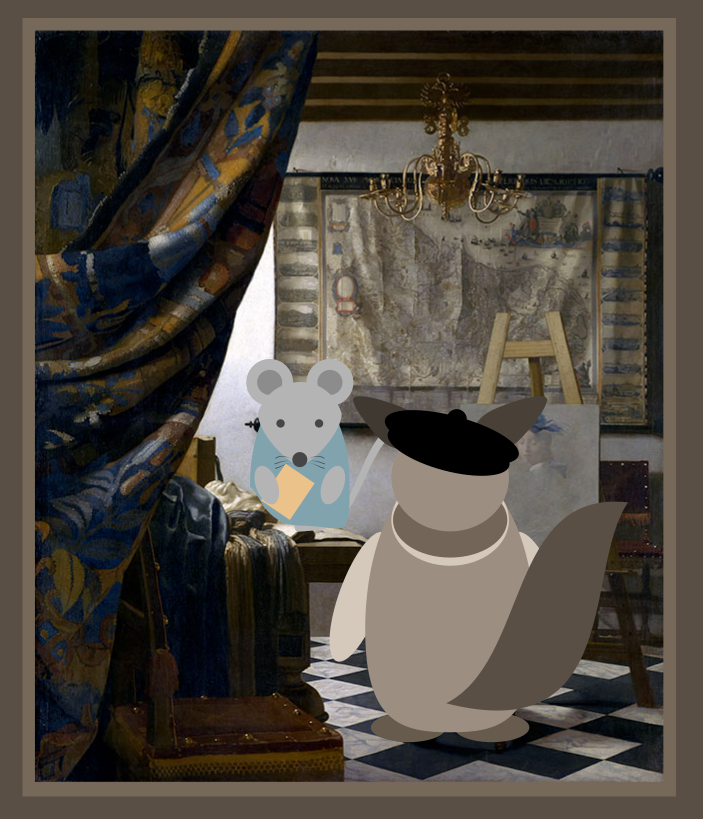
\includegraphics[height=5cm]{vermeer}};
\node at (30-0.15*\thepage,-0.4) {
\includegraphics[height=\paperheight]{rail}};
\node at (50-0.15*\thepage,0.4) {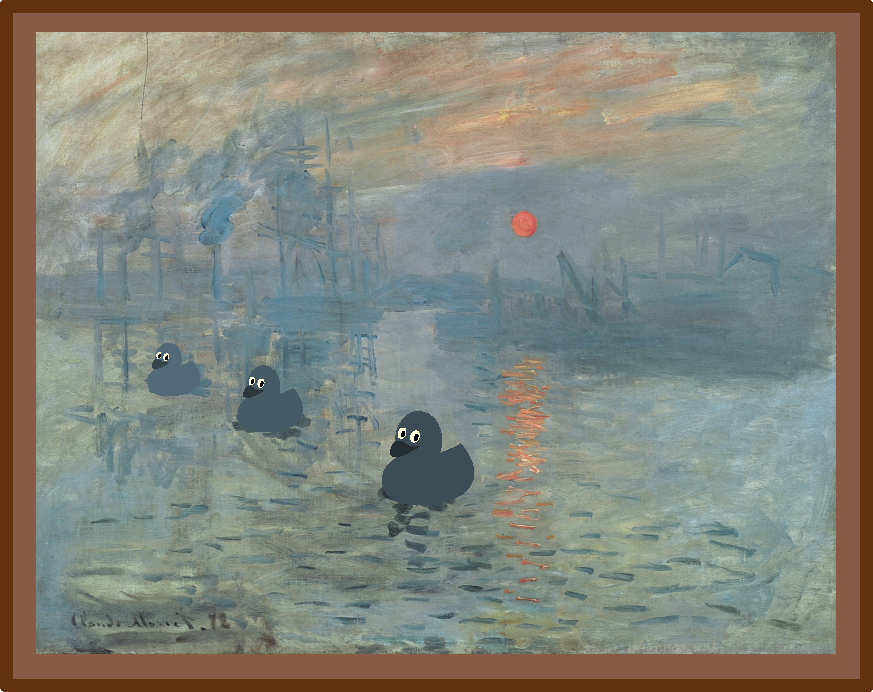
\includegraphics[height=5cm]{monet}};
\node at (60-0.15*\thepage,-0.4) {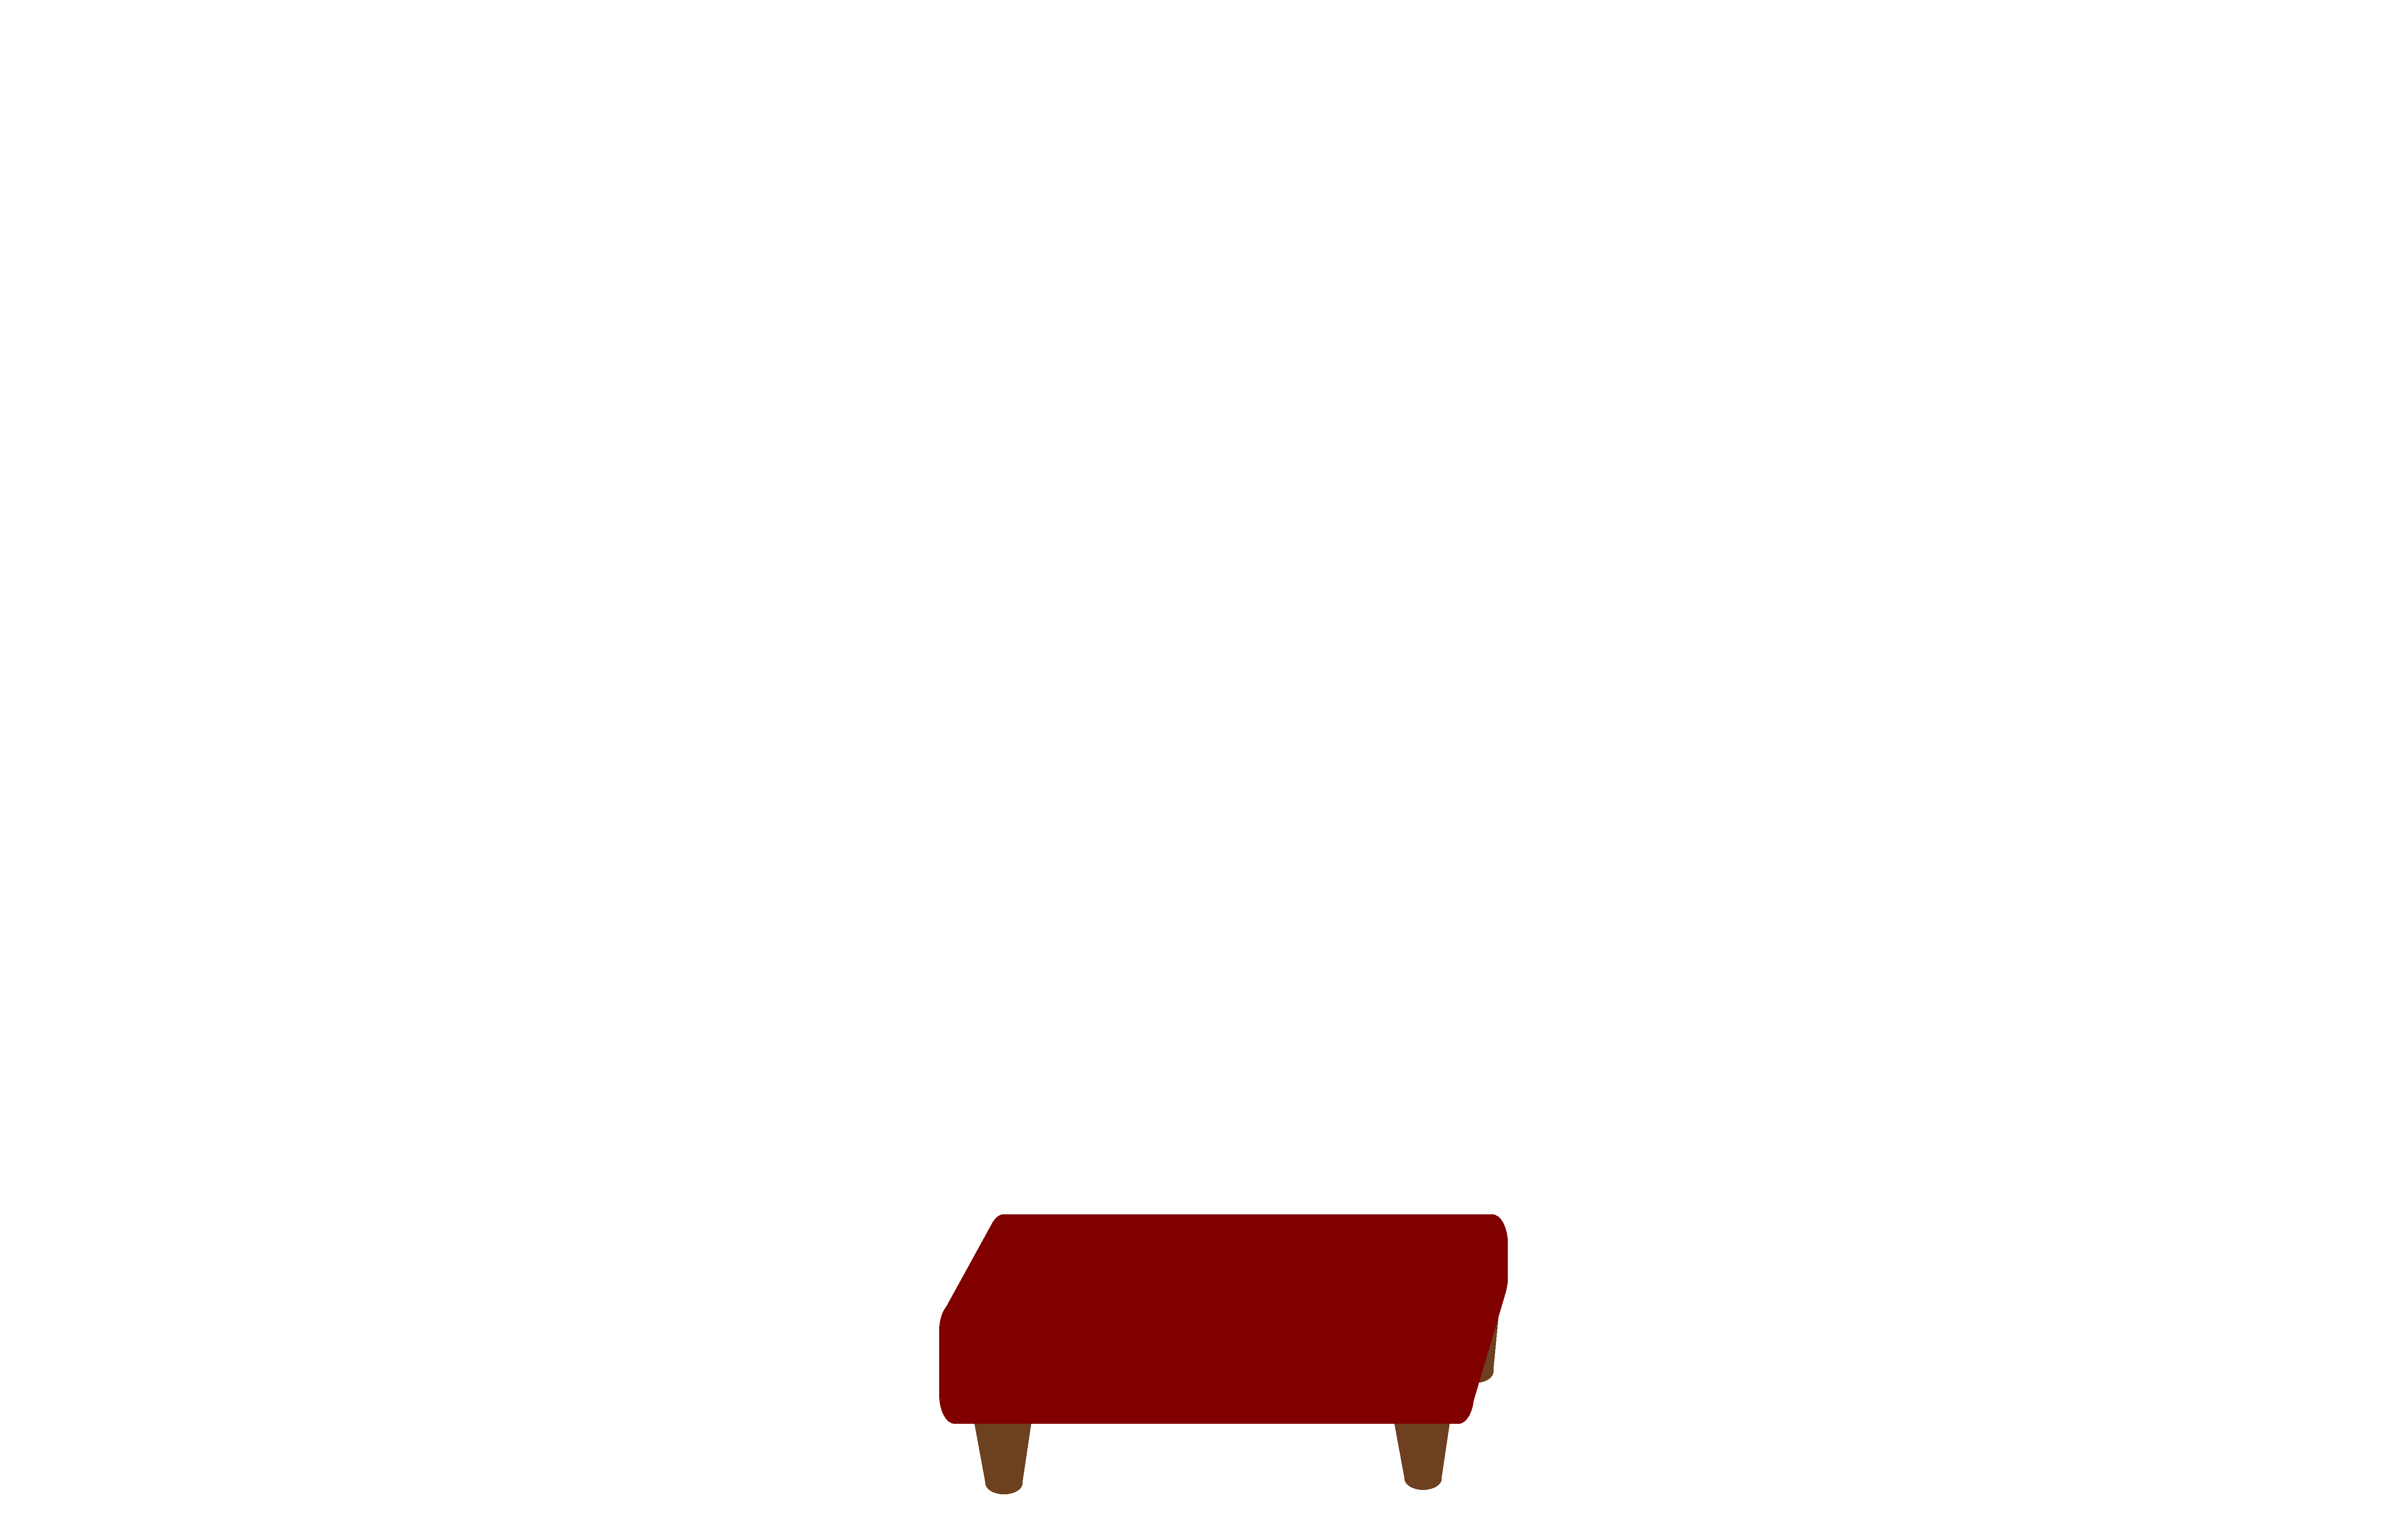
\includegraphics[height=\paperheight]{sofa}};
\node at (70-0.15*\thepage,0.4) {
\includegraphics[height=5cm]{mondrian}};
\node at (90-0.15*\thepage,0.4) {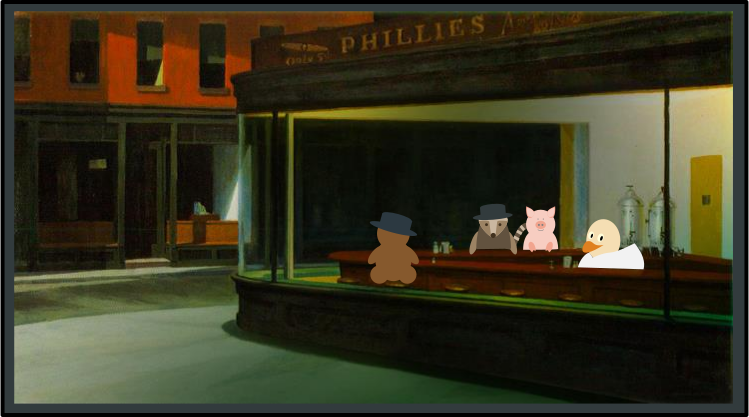
\includegraphics[height=5cm]{hopper}};
\tourist
\end{tikzpicture}
\pause[650]
\end{frame}
	
\end{document}